
\documentclass[english]{article}
\usepackage{latexsym,amsmath,amssymb,amsfonts,fullpage,graphicx,placeins}
\usepackage[capposition=top]{floatrow}

\begin{document}
Gabrielle Merritt 
\\
gmerritt@seas.upenn.edu 
\begin{center}
{\textbf{ESE 505 Homework 5}} \\
\end{center}
\section*{Design Lead lag Compensator}
\begin{equation}
G_c(s) = K \frac{s+z}{s +p} \frac{T_1s +1 }{T_2s +1}
\end{equation}
I set z and p equal to 1 to find the appropriate times to find the phase margin. 
We can rewrite $G_c(s) $ as 
$$ G_c(s)  = K*1 * \frac{s + a}{\alpha s + a } $$ 
where a is $\frac{\omega_crossover}{ 4.5} $ and $\alpha  = \frac{a}{\omega_crossover * 4.5} $ 

I then adjusted the gain to be close to the requirements 
and ended up with a z of .15 and a p of .05 
\begin{figure}[h!]
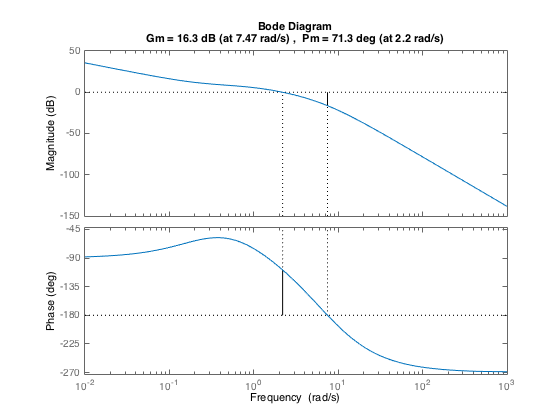
\includegraphics[width = \linewidth]{1a.png}
\caption{Bode Plot of system }
\end{figure}
\begin{figure}[h!]
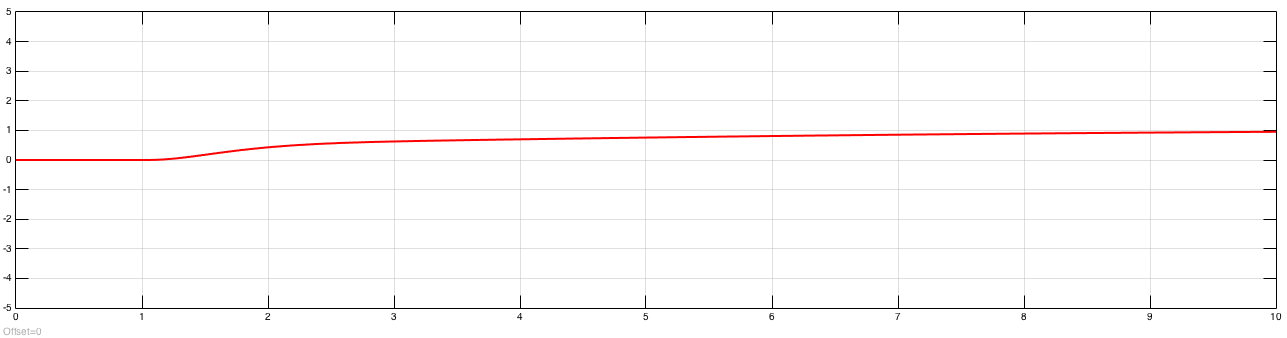
\includegraphics[width = \linewidth]{1b.png}
\caption{Step response using $G_c(S)$ Closed Loop Response}
\end{figure}
\FloatBarrier

\section*{Closed Loop Bode Plot}
\subsection*{P+I Controller} 
\paragraph*{Velocity error constant}
To take care of our velocity error constant  we can write  our controller  as $G_k(s)$ as 
$$ G_k = s \big( (\frac{K_i}{s} + K_p )(\frac{5}{2s + 1})\big) = 20 
$$
... 
$$
\lim_{s->0} K_i *5 = 20  
$$
There fore we have $K_i$ = 4 
I ignored the time delay because using the Pade approximation it simplifies when we take the limit it simplifies to 1. 
\paragraph*{Gain Margin}
 To satisfy the gain margin using Ziegler Nichols tuning method for a PI controller  $K_u$ should be equal to the gain margin 
 $$ K_p = .45 *K_u  = 2.7 
 $$

Now that we have our gains we can make a bode plot. 
To make this plot I used a first order pade approximation for the time 
\begin{figure}[!ht]
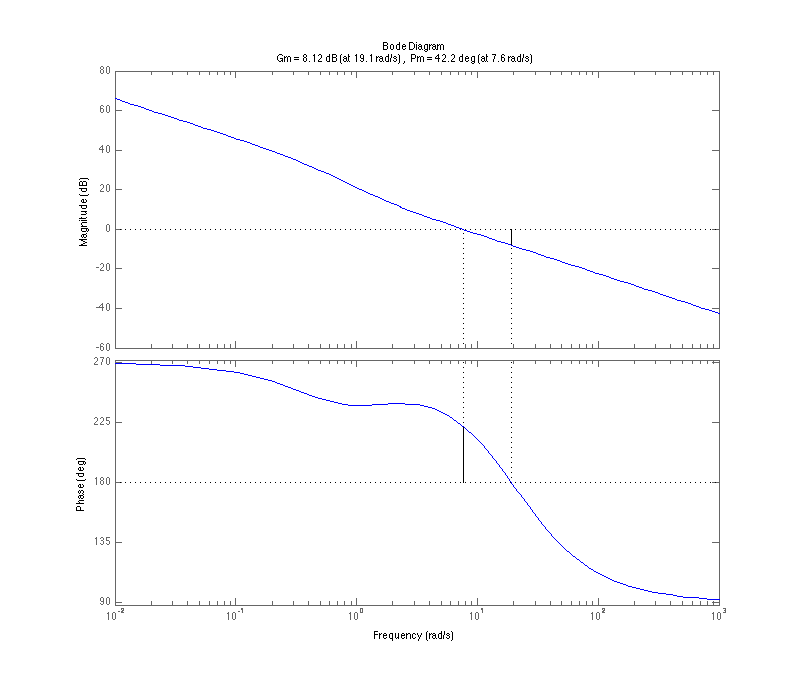
\includegraphics[width = \linewidth]{2a.png}
\caption{Open Loop Bode Plot, $\omega_c = 7.6$}
\end{figure}
\FloatBarrier 
\subsection*{Closed Loop Transfer Function}
\FloatBarrier
As we can see in figure~\ref{fig:2_b} the bandwidth frequency occurs at 17.6 radians per second.
\begin{figure}[!ht]
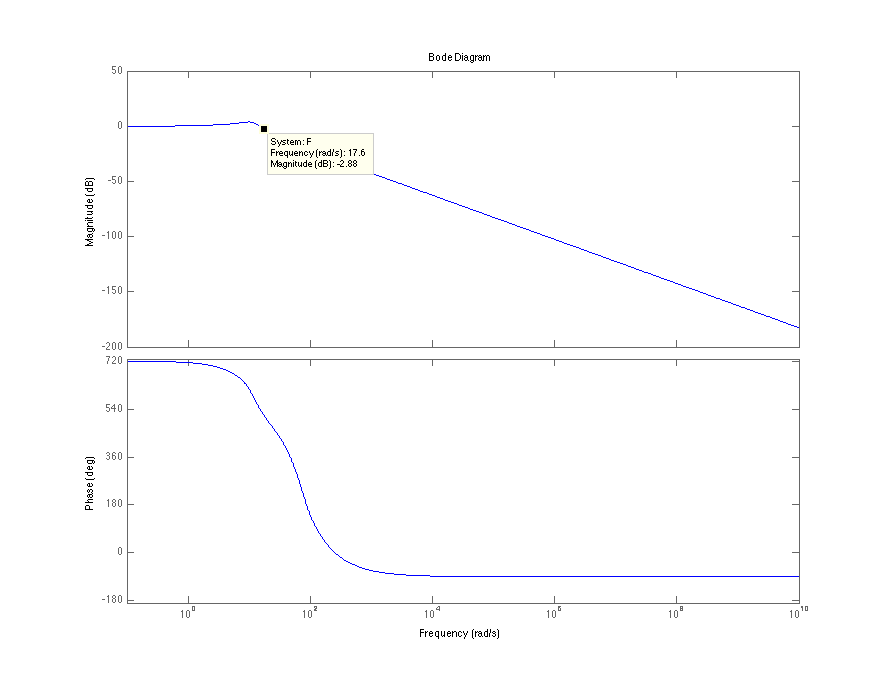
\includegraphics[width = \linewidth]{2b.png}
\caption{Closed Loop Bode Plot, $\omega_bandwidth~ 17.6 rps$}
\label{fig:2_b}
\end{figure}
\FloatBarrier 

\subsection*{What are the magnitude and phase of $CL_{(G)}$ at this frequency? You should be sure that
you see how these values are related to the open-loop bode plot (from which the margins are
computed.) Do you think it makes sense to say that the output is accurately tracking the input at this
frequency? Briefly explain.}
The gain margin between the open-loop bode and the closed loop bode is about 5.24dB at 15.1 rad per second. To find the magnitude at this frequency we see that for the closed loop response we get 
$$
  |  \big( \frac{5KG(s)}{5KG(s) + (2j\omega_{180} + 1)  })\big) | 
$$
Where $KG(s) = \big( (\frac{K_i}{s} + K_p )\big)$
If we evaluate this we should have $$|G(j\omega_{180})| = -1 $$. Which corresponds to the output being 180 degrees out of phase with the input frequency. This result is usually fine for any system that is not directly controlled by the output, for instance if you needed to  read in or process the output signal; however, if the output is to be directly linked to an actuator or a physical system the inverted output might throw off the control input (like a pilot). 

\section*{One Two Red Blue}
For the one two red blue lab, my partner and I treated the joystick as a controller on velocity instead of position, I've found that when working with joysticks that its often more intuitive to use them as a control of velocity on the object than position, therefore, I don't believe our system was subject to pilot induced oscillation. Since for small displacements of the ball we don't have to use a really low gain, or a really high gain for large displacements, if we only worry about the rate the ball is moving, so if we want to hold a position we simply have the joystick go back to its default position. 

\section*{Train Lab}
\subsection*{String Stability}
We would have string stability if the condition 
$$ H(s) = \frac{V_i(s)}{V_{i-1}(s)}  \leq 1 
$$ 
This suggests that the velocity of both trains much always match or the  velocity of the i-th train must be less than the train ahead of it. For true string stability since we want to maintain a fixed distance this condition would be almost impossible to meet since any acceleration in the previous train would require instantaneous acceleration of the next train or else the next train will always increase distance between the train ahead of it. 

When we worked on the train lab we effectively tried to have a controller on velocity of the train system, and integrated it to get position in our feedback loop. As a result our block simulink model is as follows.
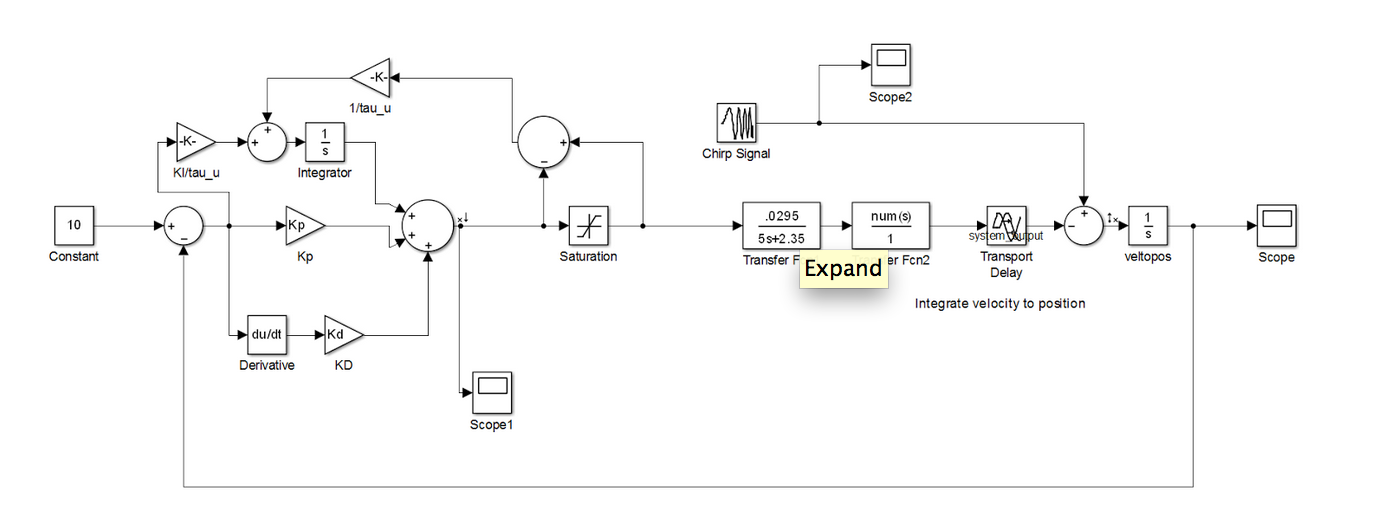
\includegraphics[width = \linewidth]{simlink.png}
\FloatBarrier
\end{document}
